\chapter{Finding Similar Item: Locality-Sensitive Hashing}
Corresponding textbook:  Chapter 3 of \href{http://www.mmds.org/}{Mining Massive Datasets}


\section{Intro} 
Given high dimensional large volume data points $x_1, ...$ and some distance function $d(x_1, x_2)$. We want to
    \begin{enumerate}
        \item Given $q$, find data points $x_j$ that are within distance threshold $d(q, x_j) \leq s$ (How to do this less than $O(N)$
        \item Find all pairs of data points $(x_i, x_j)$ that are within distance threshold $d(x_i, x_j) \leq s$ (How to do this less than $O(N^2)$
    \end{enumerate}

\paragraph{LSH}: is a family of related techniques. In generall it aims to hash similar items into the same bucket. LSH is not precise. Flase negatives exists, i.e.: similar items could be missed. 


\section{LSH Example: Similar Document} 


\subsection{Overall Structure} 
    \begin{enumerate}
        \item Shingling:  Converts a document into a set representation (Boolean vector). The output is the set of strings of length $k$ that appear in the document. 
        \item Min-Hashing: Convert large sets of shingles to short signatures, while preserving similarity The signatures are short integer vectors that represent the sets, and reflect their similarity. 
        \item Locality-Sensitive Hashing: Focus on pairs of signatures likely to be from similar documents. Outputs are candidate pairs of signatures for which we need to test for similarity. 
    \end{enumerate}
    

\subsection{Shingling} 
k-shingle is the same as k-gram. k-gram can be generate at either characters, words, or some other level depends on the application. \\

In order to compress long shingles, we can hash shingle into integer, e.g.: 4 bytes. So the final output of a document $D_i$ is the set of hashed values of its k-shingles $C_i = S(D_i)$.\\

Similarity of the output can be measured:  by 
    \begin{align*}
        \text{Jaccard similarity: } sim(D_1, D_2) = \frac{|C_1 \cap C_2|}{|C_1 \cup C_2|} \\
        \text{Jaccard Distance: } d(C_1, C_2) = 1 -  \frac{|C_1 \cap C_2|}{C_1 \cup C_2|}
    \end{align*}

The final output is a matrix representation of sets, with rows being set item (shingle) and columns are the documents.  Column similarity is the Jaccard similarity of the corresponding sets (b/c rows with value 1). 


\subsection{Min-Hashing} 
\paragraph{Contex} \mbox{}\\
In this step, we want to reduce the set representation to a smaller signature. The  goal is to find a hash function $h$ such that if $sim(C_1, C_2)$ is high, then with high probability $h(C_1) = h(C_2)$. 
    \begin{itemize}
        \item Note here the hashing isn't going to be exact, hence the word probability.
        \item Not all similarity metrics have a suitable hash function. For Jaccard similarity, the hash function is called Min-Hashing
    \end{itemize}

\paragraph{Min-Hashing Overview} \mbox{}\\
Given the boolean matrix post Shingling, we apply several random permutation $\pi$ to the matrix. The minhash function for column $C$ and permutation $\pi$ is the number of the first row post permutation in which column $C$ has value 1, i.e.: $h_\pi(C) = \min_\pi \pi(C)$. \\

The output of min-hashing is the signature matrix, where the columns are the set (document shingling output) and the rows are the permutation. Cell value is the minhash value for the corresponding column and permutation. The signature of the column / document is the minhash values for all the permutation. 


\paragraph{Min-Hashing Similarity} \mbox{}\\
The similarity of the signatures are the percent of the signature that two columns agree on. We can show that min-hash similarity equals to the column Jaccard similarity in expectation. Proof see \href{http://web.stanford.edu/class/cs246/slides/03-lsh.pdf}{slides}. Quick proof below: \\

Choose a random permutation $\pi$. Let $X$ Let $x$ be a doc (set of shingles), $z\in X$ is a shingle
    \begin{align*}
        & \text{It is equally likely that any $z\in X$ is mapped to the min element}\\
        & \Longrightarrow Pr(\pi(z) = min(\pi(X))) = \frac{1}{\abs{X}} \\
        & \text{Let $y$ be s.t. } \pi(y) = min(\pi(C_1 \cup C_2)) = \frac{1}{|C_1 \cup C_2|} \\
        & \text{There are } \abs{C_1 \cap C_2} \text{ number of options}. \\
        & \Longrightarrow Pr(min(\pi(C_1)) = min(\pi(C_2))) = \frac{\abs{C_1 \cap C_2}}{\abs{C_1 \cup C_2}}= sim(C_1, C_2)\\
    \end{align*}

\paragraph{Min-Hashing Implementation} \mbox{}\\
In reality, we do not permute the rows. We pick a row hashing function. If we want to have 100 signature, we want to pick $K=100$ hash function $h_i$, and the ordering under $h_i$ gives a random permutation $\pi$ of rows. The actual one-pass implementation would be 
    \begin{itemize}
        \item For each column $c$ and hash-function $h_i$, keep a slot $M(i,c)$ which is the min-hash value
        \item Initialize all $M(i,c)$ to be $\infty$
        \item Scan rows looking for 1s
            \begin{itemize}
                \item If row $j$ has 1 in column $c$
                \item For each $h_i$: $M(i,c) = min(M(i,c), h_i(j))$
            \end{itemize}
    \end{itemize}
One universal hashing function is $h_{a,b}(x) = ((ax + b) \mod p) \mod N$ where $a,b$ are random integers and $p$ is a prime number that is greater than $N$


\subsection{Locality-Sensitive Hashing}
\paragraph{key idea} \mbox{}\\
The goal is to find the documents with Jaccard similarity at least $s$. The idea is to use a hash function that tells whether $x$ and $y$ is a candidate pair for which the similarity must be evaluated. For Min-Hash matrices, we want to hash columns of signature matrix $M$ to many buckets. Each pair of documents that hashes into the same bucket is a candidate pair. 

\paragraph{Overview} \mbox{}\\
    \begin{itemize}
        \item Divide matrix $M$ (signature matrix from Min-Hashing) into $b$ bands of $r$ rows. (so $r \times b$ is the number of hash functions in the Min-hashing step. 
        \item For each band, hash its portion of each column to a hash table with $k$ buckets (make $k$ as large as possible so no collision). 
        \item Candidate column pairs are those that hash to the same bucket for $\geq 1$ bands
        \item Tune $b$ and $r$ to catch most similar pairs but few non-similar pairs. 
    \end{itemize}
    
\section{Theoretical Analysis of LSH} \mbox{}\\
Ideally, we want LSH to work like figure \ref{fig:LSH_ideal}. When the similarity is above the treshold, there is 100\% chance that the band will be hashed into the same bucket. \\

If we only have one bucket and 1 hash function, we know that $p(h(c_1) = h(c_2)) = sim(D_1, D_2)$, which is shown in figure \ref{fig:LSH_1_1}.

\begin{figure}[h]
  \centering
  \begin{minipage}[b]{5cm}
    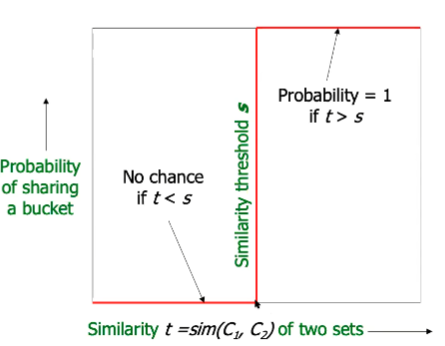
\includegraphics[width=5cm, height = 4cm]{figs/002_LSH_ideal.PNG}
    \caption{Ideal}
    \label{fig:LSH_ideal}
  \end{minipage}
  \hfill
  \begin{minipage}[b]{6cm}
    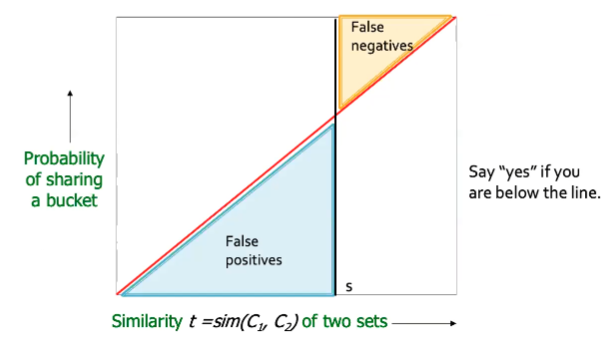
\includegraphics[width=6cm, height = 4cm]{figs/003_LSH_1_1.PNG}
    \caption{1 signature 1 band}
    \label{fig:LSH_1_1}
  \end{minipage}
\end{figure}

Now let's say we have $b$ bands and $r$ rows per band. Two columns have similarity $s$. The probability that at least 1 band is identical (becoming candidate pair) is $1 - (1 - s^r)^b$.
    \begin{itemize}
        \item The probability of a single row is the same is $s$
        \item The probability of of all rows the are the same in a band is $s^r$
        \item The probability of some rows in the band is not the same is $1 - s^r$
        \item The probability that all bands are not equal is $(1 - s^r)^b$
    \end{itemize}

So given a fixed threshold $t$, we want to pick $r$ and $b$ to get the best S-curve (close to the step function). Notice different curve will have trade-off of false positive (blue region in figure \ref{fig:LSH_1_1} and false negative (yellow region). For more exploration, see \href{https://www.desmos.com/calculator/lzzvfjiujn}{demo}. 


\section{Generalizing Min-hash to Locality Sensitive Hash Function} 
In the previous example, our input is a series of documents. We use shingling to transform the document,  use Jaccard similarity / distance as the metrics, and use min-hash function to generate the key signature. Now, we want to generalize the distance + hash function to generate signatures. 

\subsection{Distance Measure}
Let $d(\cdot)$ is a distance measure if it is a function from pairs of points $x, y$ to a real number s.t.
    \begin{itemize}
        \item $d(x,y)\geq 0$
        \item $d(x,y) = 0 \qquad iff x=y$
        \item $d(x,y) = d(y,x)$
        \item $d(x,y) \leq d(x,z) + d(z,y)$ Triangle inequality. 
    \end{itemize}

Some common distance measurement includes
    \begin{itemize}
        \item Jaccard distance: $1 - \text{Jaccard similarity}$
        \item Cosin distance: Angle between the vectors, $1 - \frac{A \cdot B}{\norm{A}\norm{B}}$
        \item Euclidean distance 
            \begin{itemize}
                \item $L_2$ norm (square root of the sum of the square of the difference in each dimension)
                \item $L_1$ norm (sum of absolute value of the difference in each dimension)
            \end{itemize}
        \item Edit distance: The minimum number of deletion / insertion to make two sequence equal. Alternative definition is $len(x) + len(y) - 2 * LCS$ (Longest common subsequence)
        \item Hamming Distance: The number of components that is different. 
    \end{itemize}



\subsection{Locality-Sensitive Families for Hash Function}
Suppose we have space $S$ of points with a distance measure $d(x,y)$. A family $H$ of hash functions (means we can effectively pick one at random and they do the same) is said to be $(d_1, d_2, p_1, p_2)-$sensitive if for any $x,y$ in $S$: 
    \begin{itemize}
        \item $d(x,y) \leq d_1 \Longrightarrow p(h(x) = h(y))\geq p_1  \qquad \forall h\in H$. 
        \item $d(x,y) \geq d_2 \Longrightarrow p(h(x) = h(y))\leq p_2  \qquad \forall h\in H$. 
    \end{itemize}
    
\subsubsection{Example: Jaccard similarity + Min-Hashing} 
Given Jaccard distance, let $d(x,y) \leq d_1$. So we know that $sim(x,y) = 1 - d(x,y) \geq 1 - d_1$. We know that the probability of min-hash function signatures agrees is same as Jaccard similarity.  

\subsection{Stacking LSH Families} 
\subsubsection{AND Construction}
Given a $(d_1, d_2, p_1, p_2)$-sensitive family $F$. We can construct a new family $F'$ by the AND construction. $f'\in F'$ is constructed from
taking the logical "and" of $r$ set of functions from $F$:  $\{f_1, ..., f_r \}$. So $f'(x) = f'(y)$ iff all $f_i$ agrees. \\

The $f'\in F'$ is $(d_1, d_2, p_1^r, p_2^r)$ 


\subsubsection{OR Construction}
Similar to and construction. \\

The $f\in F'$ is $(d_1, d_2, 1 - (1-p_1)^r, 1-(1-p_2)^r)$-sensitive. 

\subsubsection{Stacking And + OR} 
Notice "and" constructor push both probability lower, and "or" constructor push both probability higher. But they push to a different degree. So we can achieve a better outcome by stacking them, which would require more computation. \\

For example, if $F$ is $(0.2, 0.6, 0.8, 0.4)$-sensitive. We can construct $F_1$ by using 4 and "and" constructor. We have $F_1$ is $(0.2, 0.6, 0.4096, 0.0256)$-sensitive. We then construct $F_2$ to be using 4 and "or" constructor, so $F_2$ is $(0.2, 0.6, 0.878, 0.0985)$. So comparing to the original $F$, we have both better false negative $(1-0.8) > (1 - 0.878)$ and better false positive $(0.4 > 0.0985)$

\section{LSH Families for Hamming Distance} 
$f_i(x,y)$ is just the indicator function on whether the $i$th component of the vector is the same. The family $F$ is $(d_1, d_2, 1 - \frac{d_1}{d}, 1 - \frac{d_2}{d})$-sensitive. The only limitations are 1) Hamming distance runs from $0$ to $d$ instead of 0 to 1, so we need to standardize. 2) There is only $d$ number of functions in $F$.  

\section{LSH Families for Cosine Distance} 
Let vector $x, y$ construct a plane $A$ and $\theta$ be the angle between those two vectors on the plane. Consider a hyperplane $B$ represented by the projection vector $v$. If the intersection of $A$ and $B$ is between vector $x,y$, then the dot product of $v \cdot x$ and $v \dot y$ will have different sign. Otherwise, the dot product will have the same sign. Since all angles are equally likely, so the probability that the dot product will have different sign is $\frac{\theta}{180}$. 

So we can construction hash function $f\in F$ by picking a random vector $v_f$, and $f(x) = f(y)$ only if the dot product with $v_f$ has the same sign. $F$ is $(d_1, d_2, \frac{180-d_1}{180}, \frac{180-d_2}{180}$-sensitive. 

\paragraph{Sketches} Now instead of choosing random vector, we can restrict our choices to vector with component that is only $1$ or $-1$. When picking a series of those vectors and compute the sign of the dot product with $x$, the result is called sketches of $x$.  The percentage of sketches of $x$ agree with sketches of $y$ is the $\frac{\theta}{180}$ provided with enough vectors in sketches. 

\section{LSH Families for Euclidean Distance} 
Randomly pick a line, assuming the smaller angle between that line and $(x,y)$ is $\theta$. We divide the line into equally spaced bucket with $\alpha$. 

If $d(x,y)$ is smaller than $\frac{\alpha}{2}$, then there is at least $50 \%$ chance that $x,y$ will be hashed into the same bucket. If $d(x,y) \geq 2\alpha$, then there can only be non-zero probability of hashing into the same bucket if $\cos(\theta)$ between 60 and 90 (1/3 chance) (otherwise cosine greater than 1/2). 

So overall, we know $F$ is $(\alpha/2, 2\alpha, 1/2, 1/3)$-sensitive. 




